%!TEX root = ../Final_Assignment_SP_ML4IM_2023.tex
\chapter{Discussion}
\label{ch:discussion}

As seen in chapter \ref{ch:results}, the results of the project are extremly bad, so much that there is no point in using the resulting models for any kind of further research. But the results are so bad, that for one it is unlikly that these results are representative, which means that some problems must have accured during the workflow, as well as that it is worth discussing why the results are so bad, what may have happend and what could be done to improve them. \\
Because these circumstaces this chapter will not discuss the results further, but will deal with the problems that may have caused these results.

The first point to examine would be the preprocessing of the data. There are multiple problems that could arise in this step. The most prominent would be, that the prepocessing of the videos would lead to unusable or corrupt videos files. But as shown in chapter \ref{ch:methods} the outputs are correct. Some preprocessing steps provide visually better outputs to classify insect, like the background subtraction compared to the HSV, but all results servicable to yield some results. \\
Another problem could be, that the preprocessing of the images lead to a shift in the time steps of the videos.

This leads to the bounding boxes, as a shift in the time steps could lead to issues with mapping the bounding boxes correctly. 
\begin{figure}[h]
    \centering
    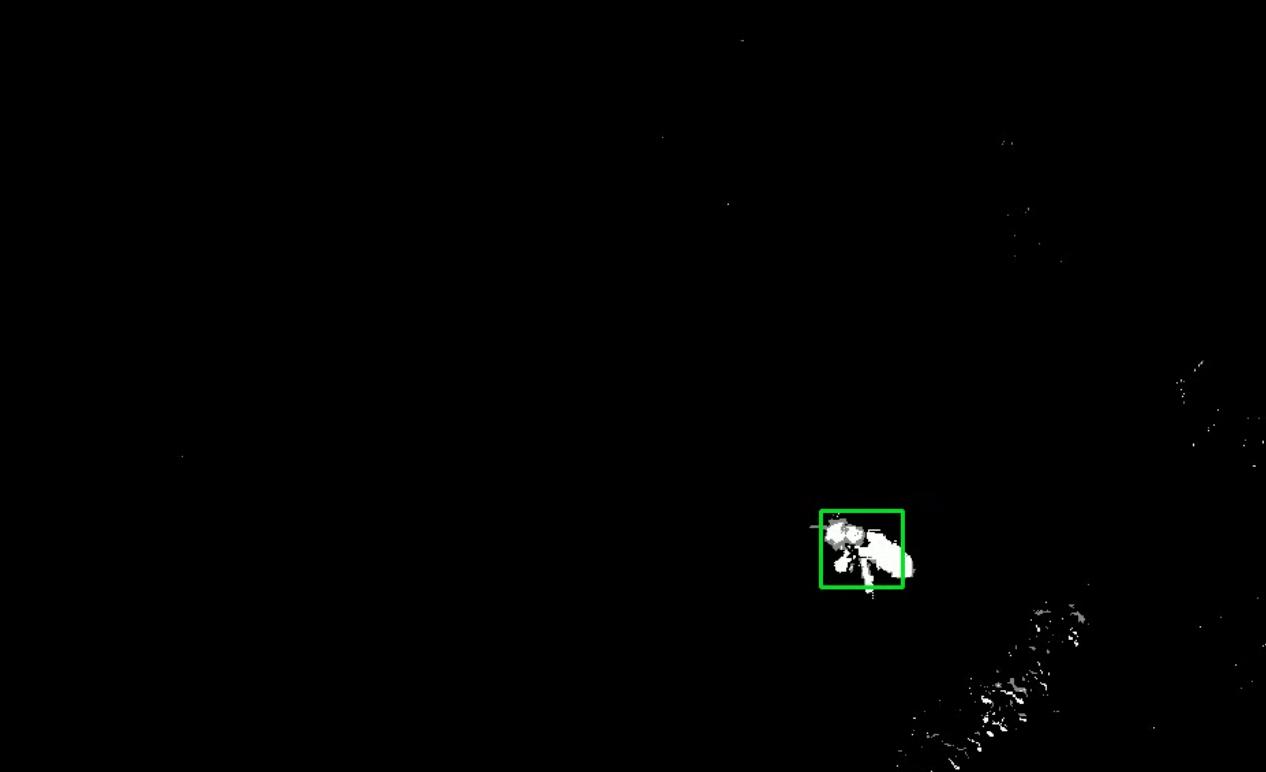
\includegraphics[width=0.5\textwidth]{images/bb_test_backSub.png}
    \caption{Combination of the preprocessed video using background subtraction and the corresponding bounding boxes}
\end{figure}

\begin{figure}[h]
    \centering
    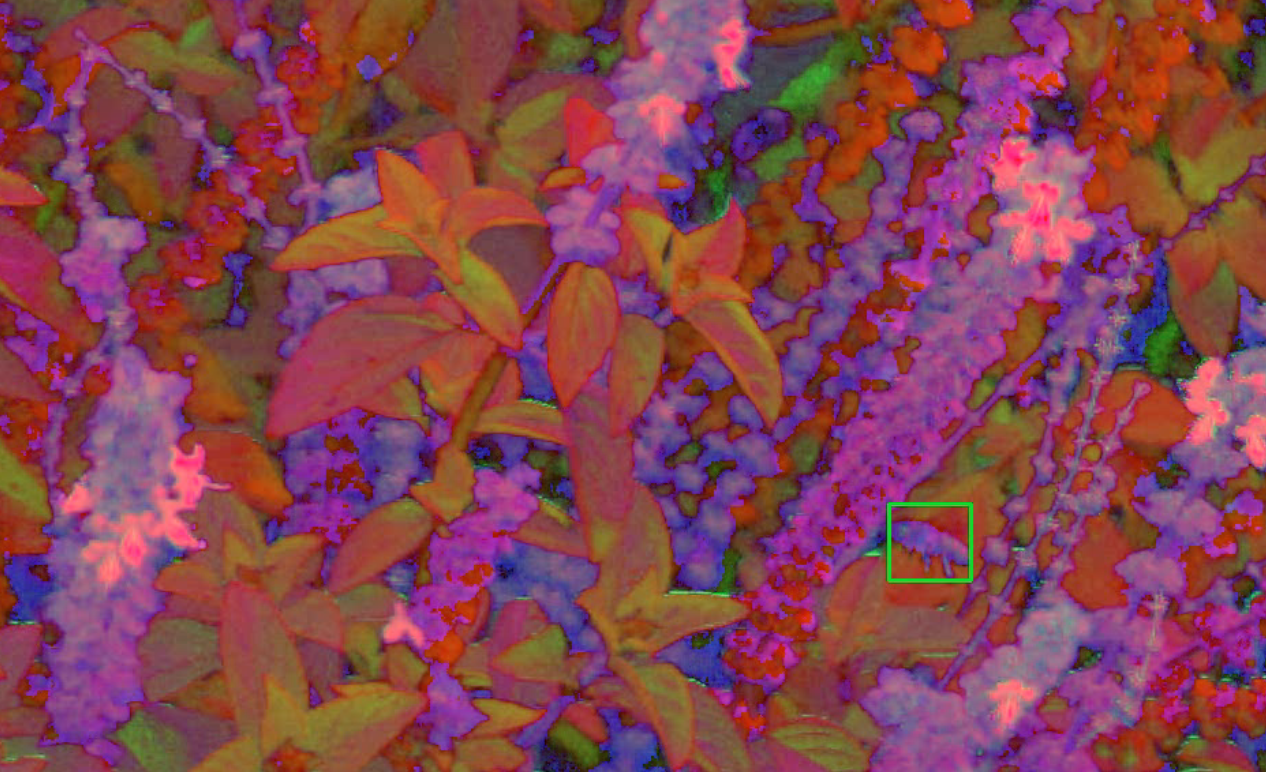
\includegraphics[width=0.5\textwidth]{images/bb_test_HSV.png}
    \caption{Combination of the preprocessed video using RGB to HSV and the corresponding bounding boxes}
\end{figure}
But as shown in the pictures above, the bounding boxes are correctly mapped to the videos. \\
As visible in the pictures the bounding boxes are not perfect and could be improved, but they are good enought to be used for training a model. The improvement of the bounding boxes could lead to minimal better results if you want to improve a already good model, but in this case the bounding boxes are not the problem.

As these points are not the problem, the next point to examine would be the training of the model. \\
As shown in chapter \ref{ch:methods} the training of the model was done using the YOLOv8 model. A possibility here could be that the default YOLOv8 model is not suitable to identify insects in the RGB or our preprocessed videos. But considering the results of the study shown in chapter \ref{ch:related_work}, which used YOLO to identify and classify street signs in RGB videos with results up to 83.2\% in the mAP@0.5 score, it is safe to assume that the YOLOv8 model should be suitable for this task. 

All the above mentioned points were problems and approaches we checked and made sure that these are not the root of the problems. The next paragraphs will discuss some other points that could have impacted the results of the models.

A possibilty might be, that the RGB data and possible preprocessing steps do not provide resulting videos that are good enough, for the algorithm to learn sensible connections out of them. As seen in chapter \ref{ch.results} the default RGB training results in a model with an mAP@0.5 value of abou 18\% which is definetly are very low value. However it is concerning that the results of the preprocessing steps are even worse, which should not be the case, because when you visually compare the used training videos for example the background subtraction should lead to way better results. \\
Continuing on the topic of trainingdata, the amout of training data can impact the results of the model. The training data used in this project contains 34 videos. This is a very low amount of data, which could lead to overfitting or bad results in generall. \\
A possible way to conteract the issue of the low amount of training data would be to incorporate cross validation into the training process.\\
The last point to improve would have been the hyperparameter of the YOLO training. These were primarily the defaults which could be improved by using a grid search to find the best hyperparameters. But because the results were so bad, it is unlikely that the hyperparameters are the problem and the attempt was made to find the bigger issue that the exact best hyperparameters.


